% Created by tikzDevice version 0.12.3.1 on 2021-06-03 19:52:22
% !TEX encoding = UTF-8 Unicode
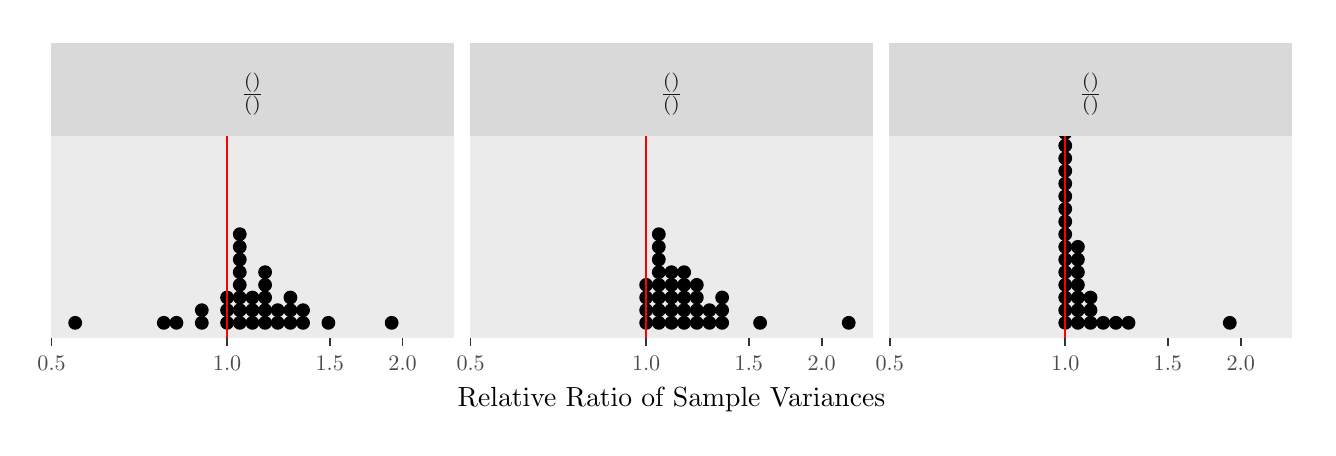
\begin{tikzpicture}[x=1pt,y=1pt]
\definecolor{fillColor}{RGB}{255,255,255}
\path[use as bounding box,fill=fillColor,fill opacity=0.00] (0,0) rectangle (462.53,144.54);
\begin{scope}
\path[clip] (  0.00,  0.00) rectangle (462.53,144.54);
\definecolor{drawColor}{RGB}{255,255,255}
\definecolor{fillColor}{RGB}{255,255,255}

\path[draw=drawColor,line width= 0.6pt,line join=round,line cap=round,fill=fillColor] (  0.00,  0.00) rectangle (462.53,144.54);
\end{scope}
\begin{scope}
\path[clip] (  8.25, 32.28) rectangle (154.18,105.24);
\definecolor{fillColor}{gray}{0.92}

\path[fill=fillColor] (  8.25, 32.28) rectangle (154.18,105.24);
\definecolor{drawColor}{RGB}{0,0,0}
\definecolor{fillColor}{RGB}{0,0,0}

\path[draw=drawColor,line width= 0.4pt,line join=round,line cap=round,fill=fillColor] ( 17.17, 37.88) circle (  2.29);

\path[draw=drawColor,line width= 0.4pt,line join=round,line cap=round,fill=fillColor] ( 49.19, 37.88) circle (  2.29);

\path[draw=drawColor,line width= 0.4pt,line join=round,line cap=round,fill=fillColor] ( 53.77, 37.88) circle (  2.29);

\path[draw=drawColor,line width= 0.4pt,line join=round,line cap=round,fill=fillColor] ( 62.92, 37.88) circle (  2.29);

\path[draw=drawColor,line width= 0.4pt,line join=round,line cap=round,fill=fillColor] ( 62.92, 42.45) circle (  2.29);

\path[draw=drawColor,line width= 0.4pt,line join=round,line cap=round,fill=fillColor] ( 72.06, 37.88) circle (  2.29);

\path[draw=drawColor,line width= 0.4pt,line join=round,line cap=round,fill=fillColor] ( 72.06, 42.45) circle (  2.29);

\path[draw=drawColor,line width= 0.4pt,line join=round,line cap=round,fill=fillColor] ( 72.06, 47.03) circle (  2.29);

\path[draw=drawColor,line width= 0.4pt,line join=round,line cap=round,fill=fillColor] ( 76.64, 37.88) circle (  2.29);

\path[draw=drawColor,line width= 0.4pt,line join=round,line cap=round,fill=fillColor] ( 76.64, 42.45) circle (  2.29);

\path[draw=drawColor,line width= 0.4pt,line join=round,line cap=round,fill=fillColor] ( 76.64, 47.03) circle (  2.29);

\path[draw=drawColor,line width= 0.4pt,line join=round,line cap=round,fill=fillColor] ( 76.64, 51.60) circle (  2.29);

\path[draw=drawColor,line width= 0.4pt,line join=round,line cap=round,fill=fillColor] ( 76.64, 56.18) circle (  2.29);

\path[draw=drawColor,line width= 0.4pt,line join=round,line cap=round,fill=fillColor] ( 76.64, 60.75) circle (  2.29);

\path[draw=drawColor,line width= 0.4pt,line join=round,line cap=round,fill=fillColor] ( 76.64, 65.33) circle (  2.29);

\path[draw=drawColor,line width= 0.4pt,line join=round,line cap=round,fill=fillColor] ( 76.64, 69.90) circle (  2.29);

\path[draw=drawColor,line width= 0.4pt,line join=round,line cap=round,fill=fillColor] ( 81.21, 37.88) circle (  2.29);

\path[draw=drawColor,line width= 0.4pt,line join=round,line cap=round,fill=fillColor] ( 81.21, 42.45) circle (  2.29);

\path[draw=drawColor,line width= 0.4pt,line join=round,line cap=round,fill=fillColor] ( 81.21, 47.03) circle (  2.29);

\path[draw=drawColor,line width= 0.4pt,line join=round,line cap=round,fill=fillColor] ( 85.79, 37.88) circle (  2.29);

\path[draw=drawColor,line width= 0.4pt,line join=round,line cap=round,fill=fillColor] ( 85.79, 42.45) circle (  2.29);

\path[draw=drawColor,line width= 0.4pt,line join=round,line cap=round,fill=fillColor] ( 85.79, 47.03) circle (  2.29);

\path[draw=drawColor,line width= 0.4pt,line join=round,line cap=round,fill=fillColor] ( 85.79, 51.60) circle (  2.29);

\path[draw=drawColor,line width= 0.4pt,line join=round,line cap=round,fill=fillColor] ( 85.79, 56.18) circle (  2.29);

\path[draw=drawColor,line width= 0.4pt,line join=round,line cap=round,fill=fillColor] ( 90.36, 37.88) circle (  2.29);

\path[draw=drawColor,line width= 0.4pt,line join=round,line cap=round,fill=fillColor] ( 90.36, 42.45) circle (  2.29);

\path[draw=drawColor,line width= 0.4pt,line join=round,line cap=round,fill=fillColor] ( 94.94, 37.88) circle (  2.29);

\path[draw=drawColor,line width= 0.4pt,line join=round,line cap=round,fill=fillColor] ( 94.94, 42.45) circle (  2.29);

\path[draw=drawColor,line width= 0.4pt,line join=round,line cap=round,fill=fillColor] ( 94.94, 47.03) circle (  2.29);

\path[draw=drawColor,line width= 0.4pt,line join=round,line cap=round,fill=fillColor] ( 99.51, 37.88) circle (  2.29);

\path[draw=drawColor,line width= 0.4pt,line join=round,line cap=round,fill=fillColor] ( 99.51, 42.45) circle (  2.29);

\path[draw=drawColor,line width= 0.4pt,line join=round,line cap=round,fill=fillColor] (108.66, 37.88) circle (  2.29);

\path[draw=drawColor,line width= 0.4pt,line join=round,line cap=round,fill=fillColor] (131.53, 37.88) circle (  2.29);
\definecolor{drawColor}{RGB}{255,0,0}

\path[draw=drawColor,line width= 0.6pt,line join=round] ( 72.06, 32.28) -- ( 72.06,105.24);
\end{scope}
\begin{scope}
\path[clip] (159.68, 32.28) rectangle (305.60,105.24);
\definecolor{fillColor}{gray}{0.92}

\path[fill=fillColor] (159.68, 32.28) rectangle (305.60,105.24);
\definecolor{drawColor}{RGB}{0,0,0}
\definecolor{fillColor}{RGB}{0,0,0}

\path[draw=drawColor,line width= 0.4pt,line join=round,line cap=round,fill=fillColor] (223.49, 37.88) circle (  2.29);

\path[draw=drawColor,line width= 0.4pt,line join=round,line cap=round,fill=fillColor] (223.49, 42.45) circle (  2.29);

\path[draw=drawColor,line width= 0.4pt,line join=round,line cap=round,fill=fillColor] (223.49, 47.03) circle (  2.29);

\path[draw=drawColor,line width= 0.4pt,line join=round,line cap=round,fill=fillColor] (223.49, 51.60) circle (  2.29);

\path[draw=drawColor,line width= 0.4pt,line join=round,line cap=round,fill=fillColor] (228.06, 37.88) circle (  2.29);

\path[draw=drawColor,line width= 0.4pt,line join=round,line cap=round,fill=fillColor] (228.06, 42.45) circle (  2.29);

\path[draw=drawColor,line width= 0.4pt,line join=round,line cap=round,fill=fillColor] (228.06, 47.03) circle (  2.29);

\path[draw=drawColor,line width= 0.4pt,line join=round,line cap=round,fill=fillColor] (228.06, 51.60) circle (  2.29);

\path[draw=drawColor,line width= 0.4pt,line join=round,line cap=round,fill=fillColor] (228.06, 56.18) circle (  2.29);

\path[draw=drawColor,line width= 0.4pt,line join=round,line cap=round,fill=fillColor] (228.06, 60.75) circle (  2.29);

\path[draw=drawColor,line width= 0.4pt,line join=round,line cap=round,fill=fillColor] (228.06, 65.33) circle (  2.29);

\path[draw=drawColor,line width= 0.4pt,line join=round,line cap=round,fill=fillColor] (228.06, 69.90) circle (  2.29);

\path[draw=drawColor,line width= 0.4pt,line join=round,line cap=round,fill=fillColor] (232.64, 37.88) circle (  2.29);

\path[draw=drawColor,line width= 0.4pt,line join=round,line cap=round,fill=fillColor] (232.64, 42.45) circle (  2.29);

\path[draw=drawColor,line width= 0.4pt,line join=round,line cap=round,fill=fillColor] (232.64, 47.03) circle (  2.29);

\path[draw=drawColor,line width= 0.4pt,line join=round,line cap=round,fill=fillColor] (232.64, 51.60) circle (  2.29);

\path[draw=drawColor,line width= 0.4pt,line join=round,line cap=round,fill=fillColor] (232.64, 56.18) circle (  2.29);

\path[draw=drawColor,line width= 0.4pt,line join=round,line cap=round,fill=fillColor] (237.21, 37.88) circle (  2.29);

\path[draw=drawColor,line width= 0.4pt,line join=round,line cap=round,fill=fillColor] (237.21, 42.45) circle (  2.29);

\path[draw=drawColor,line width= 0.4pt,line join=round,line cap=round,fill=fillColor] (237.21, 47.03) circle (  2.29);

\path[draw=drawColor,line width= 0.4pt,line join=round,line cap=round,fill=fillColor] (237.21, 51.60) circle (  2.29);

\path[draw=drawColor,line width= 0.4pt,line join=round,line cap=round,fill=fillColor] (237.21, 56.18) circle (  2.29);

\path[draw=drawColor,line width= 0.4pt,line join=round,line cap=round,fill=fillColor] (241.79, 37.88) circle (  2.29);

\path[draw=drawColor,line width= 0.4pt,line join=round,line cap=round,fill=fillColor] (241.79, 42.45) circle (  2.29);

\path[draw=drawColor,line width= 0.4pt,line join=round,line cap=round,fill=fillColor] (241.79, 47.03) circle (  2.29);

\path[draw=drawColor,line width= 0.4pt,line join=round,line cap=round,fill=fillColor] (241.79, 51.60) circle (  2.29);

\path[draw=drawColor,line width= 0.4pt,line join=round,line cap=round,fill=fillColor] (246.36, 37.88) circle (  2.29);

\path[draw=drawColor,line width= 0.4pt,line join=round,line cap=round,fill=fillColor] (246.36, 42.45) circle (  2.29);

\path[draw=drawColor,line width= 0.4pt,line join=round,line cap=round,fill=fillColor] (250.94, 37.88) circle (  2.29);

\path[draw=drawColor,line width= 0.4pt,line join=round,line cap=round,fill=fillColor] (250.94, 42.45) circle (  2.29);

\path[draw=drawColor,line width= 0.4pt,line join=round,line cap=round,fill=fillColor] (250.94, 47.03) circle (  2.29);

\path[draw=drawColor,line width= 0.4pt,line join=round,line cap=round,fill=fillColor] (264.66, 37.88) circle (  2.29);

\path[draw=drawColor,line width= 0.4pt,line join=round,line cap=round,fill=fillColor] (296.68, 37.88) circle (  2.29);
\definecolor{drawColor}{RGB}{255,0,0}

\path[draw=drawColor,line width= 0.6pt,line join=round] (223.49, 32.28) -- (223.49,105.24);
\end{scope}
\begin{scope}
\path[clip] (311.10, 32.28) rectangle (457.03,105.24);
\definecolor{fillColor}{gray}{0.92}

\path[fill=fillColor] (311.10, 32.28) rectangle (457.03,105.24);
\definecolor{drawColor}{RGB}{0,0,0}
\definecolor{fillColor}{RGB}{0,0,0}

\path[draw=drawColor,line width= 0.4pt,line join=round,line cap=round,fill=fillColor] (374.92, 37.88) circle (  2.29);

\path[draw=drawColor,line width= 0.4pt,line join=round,line cap=round,fill=fillColor] (374.92, 42.45) circle (  2.29);

\path[draw=drawColor,line width= 0.4pt,line join=round,line cap=round,fill=fillColor] (374.92, 47.03) circle (  2.29);

\path[draw=drawColor,line width= 0.4pt,line join=round,line cap=round,fill=fillColor] (374.92, 51.60) circle (  2.29);

\path[draw=drawColor,line width= 0.4pt,line join=round,line cap=round,fill=fillColor] (374.92, 56.18) circle (  2.29);

\path[draw=drawColor,line width= 0.4pt,line join=round,line cap=round,fill=fillColor] (374.92, 60.75) circle (  2.29);

\path[draw=drawColor,line width= 0.4pt,line join=round,line cap=round,fill=fillColor] (374.92, 65.33) circle (  2.29);

\path[draw=drawColor,line width= 0.4pt,line join=round,line cap=round,fill=fillColor] (374.92, 69.90) circle (  2.29);

\path[draw=drawColor,line width= 0.4pt,line join=round,line cap=round,fill=fillColor] (374.92, 74.48) circle (  2.29);

\path[draw=drawColor,line width= 0.4pt,line join=round,line cap=round,fill=fillColor] (374.92, 79.05) circle (  2.29);

\path[draw=drawColor,line width= 0.4pt,line join=round,line cap=round,fill=fillColor] (374.92, 83.62) circle (  2.29);

\path[draw=drawColor,line width= 0.4pt,line join=round,line cap=round,fill=fillColor] (374.92, 88.20) circle (  2.29);

\path[draw=drawColor,line width= 0.4pt,line join=round,line cap=round,fill=fillColor] (374.92, 92.77) circle (  2.29);

\path[draw=drawColor,line width= 0.4pt,line join=round,line cap=round,fill=fillColor] (374.92, 97.35) circle (  2.29);

\path[draw=drawColor,line width= 0.4pt,line join=round,line cap=round,fill=fillColor] (374.92,101.92) circle (  2.29);

\path[draw=drawColor,line width= 0.4pt,line join=round,line cap=round,fill=fillColor] (374.92,106.50) circle (  2.29);

\path[draw=drawColor,line width= 0.4pt,line join=round,line cap=round,fill=fillColor] (374.92,111.07) circle (  2.29);

\path[draw=drawColor,line width= 0.4pt,line join=round,line cap=round,fill=fillColor] (374.92,115.65) circle (  2.29);

\path[draw=drawColor,line width= 0.4pt,line join=round,line cap=round,fill=fillColor] (374.92,120.22) circle (  2.29);

\path[draw=drawColor,line width= 0.4pt,line join=round,line cap=round,fill=fillColor] (379.49, 37.88) circle (  2.29);

\path[draw=drawColor,line width= 0.4pt,line join=round,line cap=round,fill=fillColor] (379.49, 42.45) circle (  2.29);

\path[draw=drawColor,line width= 0.4pt,line join=round,line cap=round,fill=fillColor] (379.49, 47.03) circle (  2.29);

\path[draw=drawColor,line width= 0.4pt,line join=round,line cap=round,fill=fillColor] (379.49, 51.60) circle (  2.29);

\path[draw=drawColor,line width= 0.4pt,line join=round,line cap=round,fill=fillColor] (379.49, 56.18) circle (  2.29);

\path[draw=drawColor,line width= 0.4pt,line join=round,line cap=round,fill=fillColor] (379.49, 60.75) circle (  2.29);

\path[draw=drawColor,line width= 0.4pt,line join=round,line cap=round,fill=fillColor] (379.49, 65.33) circle (  2.29);

\path[draw=drawColor,line width= 0.4pt,line join=round,line cap=round,fill=fillColor] (384.06, 37.88) circle (  2.29);

\path[draw=drawColor,line width= 0.4pt,line join=round,line cap=round,fill=fillColor] (384.06, 42.45) circle (  2.29);

\path[draw=drawColor,line width= 0.4pt,line join=round,line cap=round,fill=fillColor] (384.06, 47.03) circle (  2.29);

\path[draw=drawColor,line width= 0.4pt,line join=round,line cap=round,fill=fillColor] (388.64, 37.88) circle (  2.29);

\path[draw=drawColor,line width= 0.4pt,line join=round,line cap=round,fill=fillColor] (393.21, 37.88) circle (  2.29);

\path[draw=drawColor,line width= 0.4pt,line join=round,line cap=round,fill=fillColor] (397.79, 37.88) circle (  2.29);

\path[draw=drawColor,line width= 0.4pt,line join=round,line cap=round,fill=fillColor] (434.38, 37.88) circle (  2.29);
\definecolor{drawColor}{RGB}{255,0,0}

\path[draw=drawColor,line width= 0.6pt,line join=round] (374.92, 32.28) -- (374.92,105.24);
\end{scope}
\begin{scope}
\path[clip] (  8.25,105.24) rectangle (154.18,139.04);
\definecolor{fillColor}{gray}{0.85}

\path[fill=fillColor] (  8.25,105.24) rectangle (154.18,139.04);
\definecolor{drawColor}{gray}{0.10}

\node[text=drawColor,anchor=base,inner sep=0pt, outer sep=0pt, scale=  1.00] at ( 81.21,125.21) {};

\node[text=drawColor,anchor=base,inner sep=0pt, outer sep=0pt, scale=  1.00] at ( 81.21,118.01) {$\frac{\varhat(\tsd)}{\varhat(\trebar)}$};

\node[text=drawColor,anchor=base,inner sep=0pt, outer sep=0pt, scale=  1.00] at ( 81.21,110.81) {};
\end{scope}
\begin{scope}
\path[clip] (159.68,105.24) rectangle (305.60,139.04);
\definecolor{fillColor}{gray}{0.85}

\path[fill=fillColor] (159.68,105.24) rectangle (305.60,139.04);
\definecolor{drawColor}{gray}{0.10}

\node[text=drawColor,anchor=base,inner sep=0pt, outer sep=0pt, scale=  1.00] at (232.64,125.21) {};

\node[text=drawColor,anchor=base,inner sep=0pt, outer sep=0pt, scale=  1.00] at (232.64,118.01) {$\frac{\varhat(\tsd)}{\varhat(\trc)}$};

\node[text=drawColor,anchor=base,inner sep=0pt, outer sep=0pt, scale=  1.00] at (232.64,110.81) {};
\end{scope}
\begin{scope}
\path[clip] (311.10,105.24) rectangle (457.03,139.04);
\definecolor{fillColor}{gray}{0.85}

\path[fill=fillColor] (311.10,105.24) rectangle (457.03,139.04);
\definecolor{drawColor}{gray}{0.10}

\node[text=drawColor,anchor=base,inner sep=0pt, outer sep=0pt, scale=  1.00] at (384.06,125.21) {};

\node[text=drawColor,anchor=base,inner sep=0pt, outer sep=0pt, scale=  1.00] at (384.06,118.01) {$\frac{\varhat(\trebar)}{\varhat(\trc)}$};

\node[text=drawColor,anchor=base,inner sep=0pt, outer sep=0pt, scale=  1.00] at (384.06,110.81) {};
\end{scope}
\begin{scope}
\path[clip] (  0.00,  0.00) rectangle (462.53,144.54);
\definecolor{drawColor}{gray}{0.20}

\path[draw=drawColor,line width= 0.6pt,line join=round] (  8.65, 29.53) --
	(  8.65, 32.28);

\path[draw=drawColor,line width= 0.6pt,line join=round] ( 72.06, 29.53) --
	( 72.06, 32.28);

\path[draw=drawColor,line width= 0.6pt,line join=round] (109.16, 29.53) --
	(109.16, 32.28);

\path[draw=drawColor,line width= 0.6pt,line join=round] (135.48, 29.53) --
	(135.48, 32.28);
\end{scope}
\begin{scope}
\path[clip] (  0.00,  0.00) rectangle (462.53,144.54);
\definecolor{drawColor}{gray}{0.30}

\node[text=drawColor,anchor=base,inner sep=0pt, outer sep=0pt, scale=  0.80] at (  8.65, 20.71) {0.5};

\node[text=drawColor,anchor=base,inner sep=0pt, outer sep=0pt, scale=  0.80] at ( 72.06, 20.71) {1.0};

\node[text=drawColor,anchor=base,inner sep=0pt, outer sep=0pt, scale=  0.80] at (109.16, 20.71) {1.5};

\node[text=drawColor,anchor=base,inner sep=0pt, outer sep=0pt, scale=  0.80] at (135.48, 20.71) {2.0};
\end{scope}
\begin{scope}
\path[clip] (  0.00,  0.00) rectangle (462.53,144.54);
\definecolor{drawColor}{gray}{0.20}

\path[draw=drawColor,line width= 0.6pt,line join=round] (160.07, 29.53) --
	(160.07, 32.28);

\path[draw=drawColor,line width= 0.6pt,line join=round] (223.49, 29.53) --
	(223.49, 32.28);

\path[draw=drawColor,line width= 0.6pt,line join=round] (260.59, 29.53) --
	(260.59, 32.28);

\path[draw=drawColor,line width= 0.6pt,line join=round] (286.91, 29.53) --
	(286.91, 32.28);
\end{scope}
\begin{scope}
\path[clip] (  0.00,  0.00) rectangle (462.53,144.54);
\definecolor{drawColor}{gray}{0.30}

\node[text=drawColor,anchor=base,inner sep=0pt, outer sep=0pt, scale=  0.80] at (160.07, 20.71) {0.5};

\node[text=drawColor,anchor=base,inner sep=0pt, outer sep=0pt, scale=  0.80] at (223.49, 20.71) {1.0};

\node[text=drawColor,anchor=base,inner sep=0pt, outer sep=0pt, scale=  0.80] at (260.59, 20.71) {1.5};

\node[text=drawColor,anchor=base,inner sep=0pt, outer sep=0pt, scale=  0.80] at (286.91, 20.71) {2.0};
\end{scope}
\begin{scope}
\path[clip] (  0.00,  0.00) rectangle (462.53,144.54);
\definecolor{drawColor}{gray}{0.20}

\path[draw=drawColor,line width= 0.6pt,line join=round] (311.50, 29.53) --
	(311.50, 32.28);

\path[draw=drawColor,line width= 0.6pt,line join=round] (374.92, 29.53) --
	(374.92, 32.28);

\path[draw=drawColor,line width= 0.6pt,line join=round] (412.01, 29.53) --
	(412.01, 32.28);

\path[draw=drawColor,line width= 0.6pt,line join=round] (438.33, 29.53) --
	(438.33, 32.28);
\end{scope}
\begin{scope}
\path[clip] (  0.00,  0.00) rectangle (462.53,144.54);
\definecolor{drawColor}{gray}{0.30}

\node[text=drawColor,anchor=base,inner sep=0pt, outer sep=0pt, scale=  0.80] at (311.50, 20.71) {0.5};

\node[text=drawColor,anchor=base,inner sep=0pt, outer sep=0pt, scale=  0.80] at (374.92, 20.71) {1.0};

\node[text=drawColor,anchor=base,inner sep=0pt, outer sep=0pt, scale=  0.80] at (412.01, 20.71) {1.5};

\node[text=drawColor,anchor=base,inner sep=0pt, outer sep=0pt, scale=  0.80] at (438.33, 20.71) {2.0};
\end{scope}
\begin{scope}
\path[clip] (  0.00,  0.00) rectangle (462.53,144.54);
\definecolor{drawColor}{RGB}{0,0,0}

\node[text=drawColor,anchor=base,inner sep=0pt, outer sep=0pt, scale=  1.00] at (232.64,  7.83) {Relative Ratio of Sample Variances};
\end{scope}
\end{tikzpicture}
